\documentclass[aspectratio = 169]{beamer}
\usetheme{CambridgeUS}
\usecolortheme{beaver}

\usepackage{graphicx}  
\usepackage{amsmath, amssymb}
\usepackage{hyperref}

\title{Michelson Experiment Summary}
\author{Yongao Hu}
\institute{MIT Department of Physics}
\date{\today}

\begin{document}

% Title Slide
\begin{frame}
    \titlepage
\end{frame}

% Outline Slide
\begin{frame}{Outline}
    \tableofcontents
\end{frame}

% Introduction Slide
\section{Introduction}
\begin{frame}{Introduction}
    \begin{itemize}
        \item Light exhibits interference when two waves overlap.
        \item The Michelson interferometer, designed by Albert Michelson, measures the wavelength of light.
        \item Historically, it disproved the existence of the "luminiferous aether" and contributed to relativity.
        \item Interferometers are used in:
        \begin{itemize}
            \item Precision measurements
            \item LIGO for detecting gravitational waves \cite{LIGO2016}
        \end{itemize}
    \end{itemize}
\end{frame}

% Theory Slide
\section{Theory}
\begin{frame}{Interference of Light Waves}
    \begin{itemize}
        \item The interference pattern depends on the phase difference:
        \[
        \Delta \phi = 2\pi \frac{\Delta x}{\lambda}
        \]
        \item Intensity of interference:
        \[
        I = I_0 \cos^2(\Delta \phi)
        \]
        \item Maximum interference: $\Delta \phi = 2\pi n$
        \item Minimum interference: $\Delta \phi = (2n+1)\pi$
    \end{itemize}
\end{frame}

\begin{frame}{Visibility of the Interference Pattern}
    \begin{itemize}
        \item Visibility measures how well the pattern is resolved:
        \[
        V = \frac{I_{\text{max}} - I_{\text{min}}}{I_{\text{max}} + I_{\text{min}}}
        \]
        \item Ideal case: $V = 1$
        \item Low visibility $\Rightarrow$ poor alignment or coherence issues.
    \end{itemize}
\end{frame}

\begin{frame}{Piezoelectric Transducer for Path Difference}
    \begin{itemize}
        \item A piezoelectric transducer moves a mirror in response to voltage.
        \item This changes the path length $\Delta x$, altering the interference pattern.
        \item The wavelength of light is found using:
        \[
        \lambda = 4 \Delta V \times \frac{\Delta L}{V}
        \]
    \end{itemize}
\end{frame}

% Experimental Setup Slide
\section{Experimental Setup}
\begin{frame}{Michelson Interferometer Setup}
    \begin{itemize}
        \item Light source: laser
        \item 50/50 beam splitter splits the light into two paths.
        \item One mirror is stationary, the other mounted on a piezoelectric transducer.
        \item Detector: photodiode (voltage output proportional to intensity).
        \item Signal generator applies a triangular voltage to move the mirror.
    \end{itemize}
\end{frame}

\begin{frame}{Experimental Setup - Schematic}
    \centering
    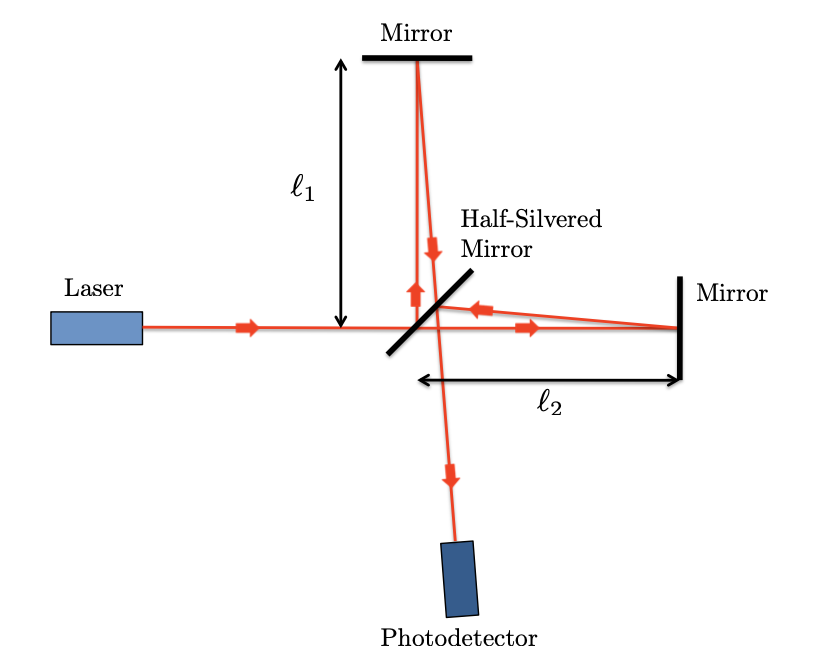
\includegraphics[width=0.7\textwidth]{fig/michelson_setup.png}
    \caption{Schematic of the Michelson interferometer. Adapted from \cite{MITOpticalInterferometry2023}.}
\end{frame}

% Data Analysis Slide
\section{Data Analysis}
\begin{frame}{Data Processing}
    \begin{itemize}
        \item Voltage signals recorded from signal generator and photodiode.
        \item Used \texttt{findpeak} in \texttt{SciPy} to locate primary maxima and minima.
        \item Applied \texttt{KMeans} clustering (\texttt{SciKit-Learn}) to group voltage values.
        \item Measured $\Delta V$ between consecutive maxima and minima.
    \end{itemize}
\end{frame}

\begin{frame}{Interference Pattern Visibility}
    \centering
    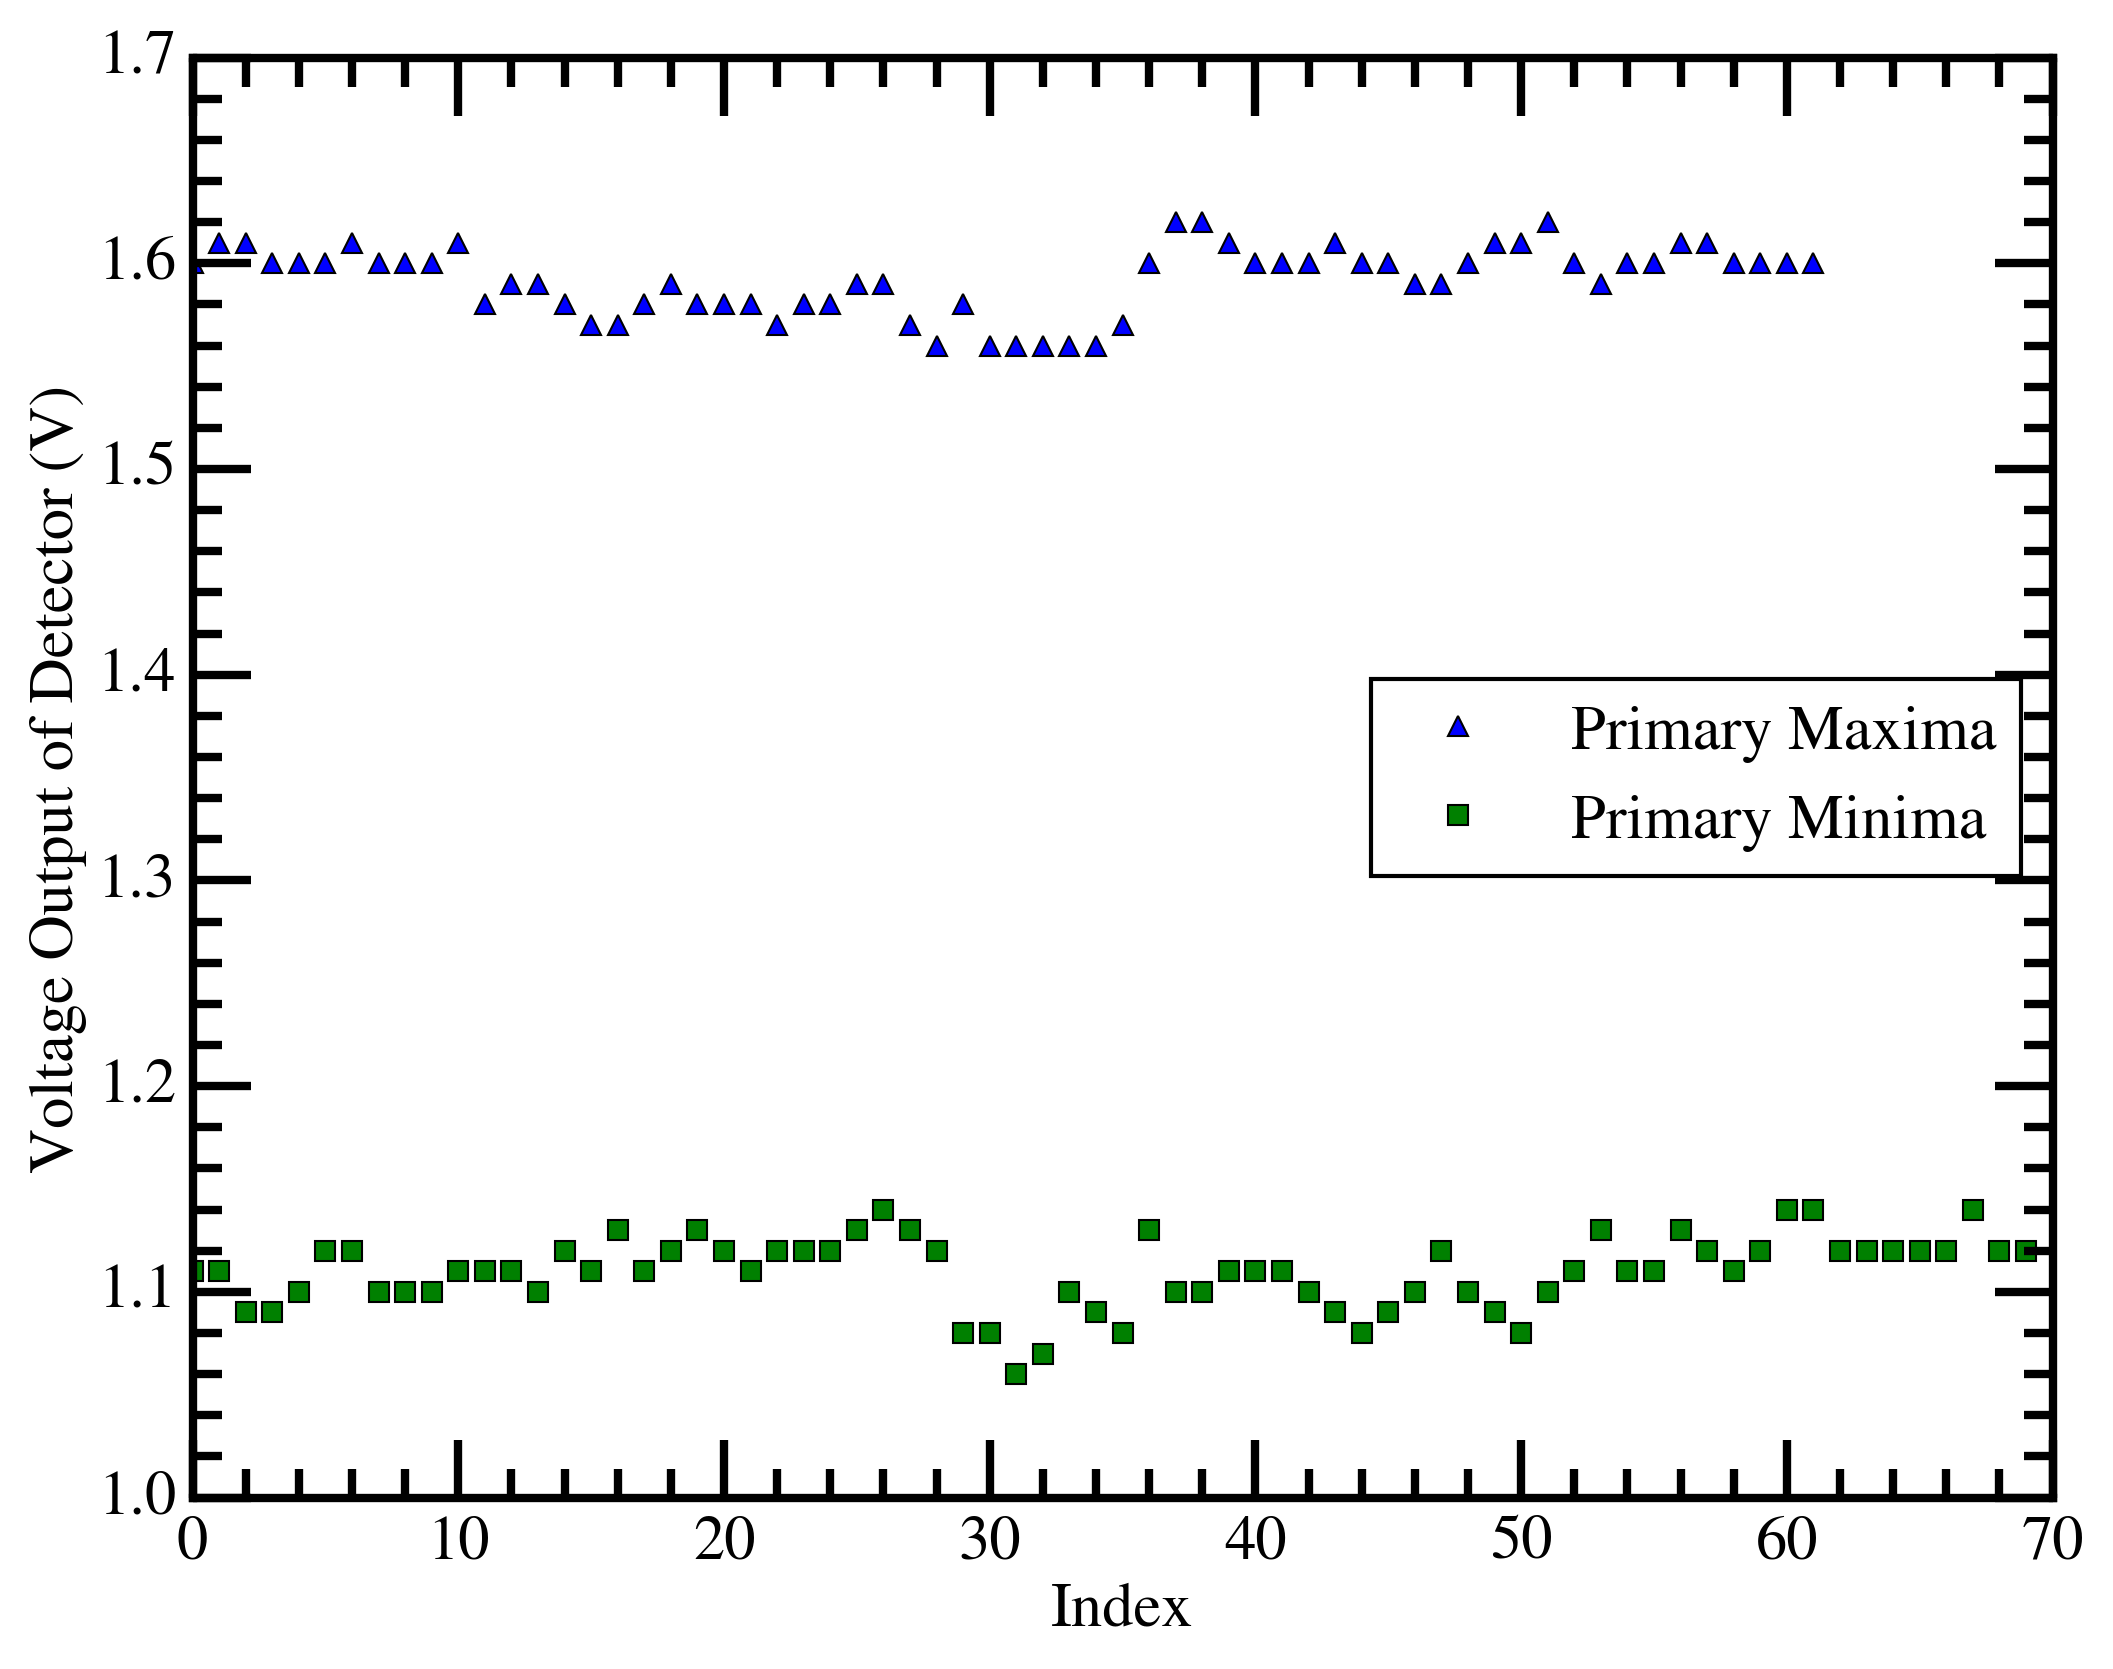
\includegraphics[width=0.7\textwidth]{fig/Intensity.png}
    \caption{Voltage output of photodiode corresponding to maxima and minima.}
\end{frame}

% Results Slide
\section{Results}
\begin{frame}{Visibility Measurement}
    \begin{itemize}
        \item Maximum voltage: $(1.592\pm0.002)\text{ V}$
        \item Minimum voltage: $(1.110\pm0.002)\text{ V}$
        \item Visibility:
        \[
        V = 0.179\pm0.001
        \]
        \item Imperfect alignment likely lowered visibility.
    \end{itemize}
\end{frame}

\begin{frame}{Wavelength Measurement}
    \begin{itemize}
        \item Measured voltage difference between peaks: $(3.192 \pm 0.055) \text{ V}$
        \item Calculated wavelength:
        \[
        \lambda = 601\pm37(\text{sys})\pm10(\text{stat})\text{ nm}
        \]
        \item Matches expected wavelength of the orange laser.
    \end{itemize}
\end{frame}

\begin{frame}{Voltage Data at Peaks}
    \centering
    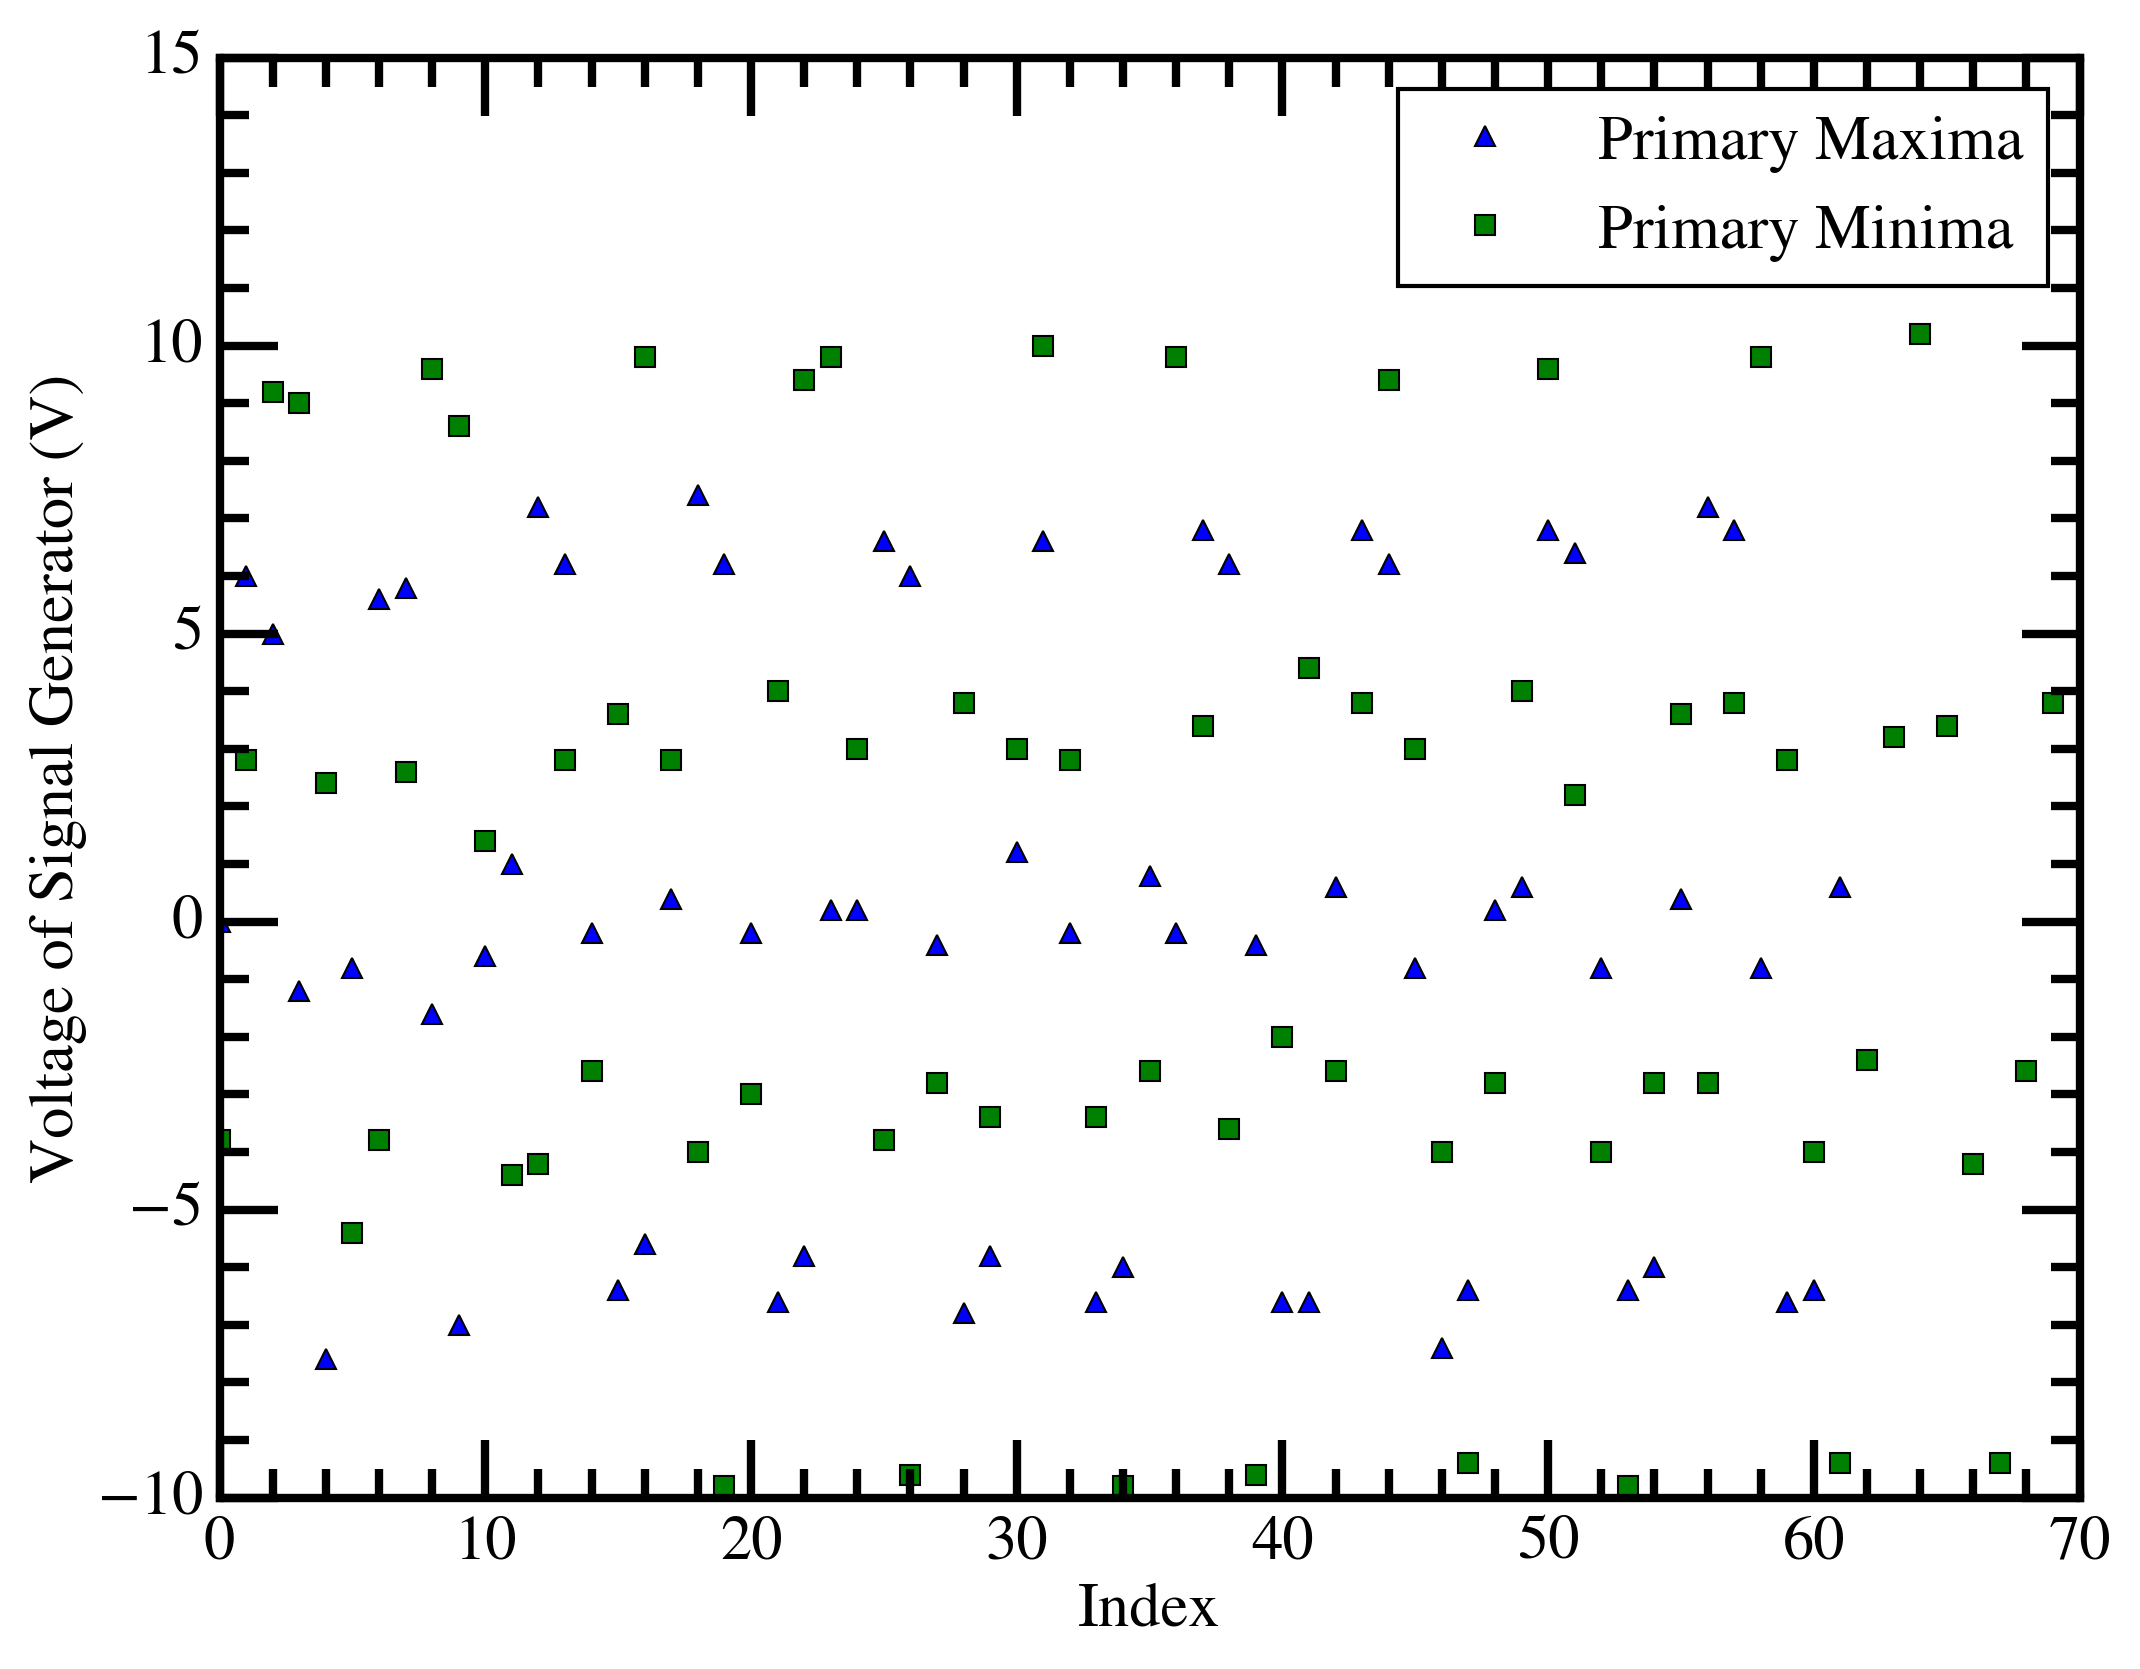
\includegraphics[width=0.7\textwidth]{fig/Primary_Maxima_Minima.png}
    \caption{Voltage at primary maxima and minima.}
\end{frame}

% Uncertainty Analysis Slide
\section{Uncertainty Analysis}
\begin{frame}{Sources of Uncertainty}
    \begin{itemize}
        \item **Systematic error**: Calibration of the piezoelectric device
        \[
        \delta \lambda = 37 \text{ nm}
        \]
        \item **Statistical error**: Peak detection noise
        \[
        \delta \lambda = 10 \text{ nm}
        \]
        \item **Total error dominated by systematic effects.**
    \end{itemize}
\end{frame}

% Conclusion Slide
\section{Conclusion}
\begin{frame}{Conclusion}
    \begin{itemize}
        \item Successfully measured the wavelength of an orange laser:
        \[
        601\pm37(\text{sys})\pm10(\text{stat})\text{ nm}
        \]
        \item Demonstrated interference and wave nature of light.
        \item Future improvements:
        \begin{itemize}
            \item Improve mirror alignment for higher visibility.
            \item Use a more precise piezoelectric transducer.
            \item Implement automated feedback to stabilize fringes.
        \end{itemize}
    \end{itemize}
\end{frame}

% Acknowledgments Slide
\begin{frame}{Acknowledgments}
    \begin{itemize}
        \item Special thanks to J. Lewis, M. Bohdan, and V. Tran for assistance.
        \item Thanks to the MIT 8.13 teaching team for guidance.
        \item Supported by the MIT Department of Physics.
    \end{itemize}
\end{frame}

% References Slide
\begin{frame}[allowframebreaks]{References}
    \bibliographystyle{unsrt}
    \bibliography{report_michelson_ref}
\end{frame}

\end{document}